%%%%%%%%%%%%%%%%%%%%%%% file template.tex %%%%%%%%%%%%%%%%%%%%%%%%%
%
% This is a general template file for the LaTeX package SVJour3
% for Springer journals.          Springer Heidelberg 2010/09/16
%
% Copy it to a new file with a new name and use it as the basis
% for your article. Delete % signs as needed.
%
% This template includes a few options for different layouts and
% content for various journals. Please consult a previous issue of
% your journal as needed.
%
%%%%%%%%%%%%%%%%%%%%%%%%%%%%%%%%%%%%%%%%%%%%%%%%%%%%%%%%%%%%%%%%%%%
%
% First comes an example EPS file -- just ignore it and
% proceed on the \documentclass line
% your LaTeX will extract the file if required
\begin{filecontents*}{example.eps}
%!PS-Adobe-3.0 EPSF-3.0
%%BoundingBox: 19 19 221 221
%%CreationDate: Mon Sep 29 1997
%%Creator: programmed by hand (JK)
%%EndComments
gsave
newpath
  20 20 moveto
  20 220 lineto
  220 220 lineto
  220 20 lineto
closepath
2 setlinewidth
gsave
  .4 setgray fill
grestore
stroke
grestore
\end{filecontents*}
%
\RequirePackage{fix-cm}
%
%\documentclass{svjour3}                     % onecolumn (standard format)
%\documentclass[smallcondensed]{svjour3}     % onecolumn (ditto)
\documentclass[smallextended]{svjour3}       % onecolumn (second format)
%\documentclass[twocolumn]{svjour3}          % twocolumn
%
\smartqed  % flush right qed marks, e.g. at end of proof
%
\usepackage{graphicx}
%
% \usepackage{mathptmx}      % use Times fonts if available on your TeX system
%
% insert here the call for the packages your document requires
%\usepackage{latexsym}
% etc.
%
% please place your own definitions here and don't use \def but
% \newcommand{}{}
%
% Insert the name of "your journal" with
% \journalname{myjournal}
%
\begin{document}

\title{Lactamotion:%\thanks{Grants or other notes
%about the article that should go on the front page should be
%placed here. General acknowledgments should be placed at the end of the article.}
}
\subtitle{Postpartum mobility in northwestern Namibia}

%\titlerunning{Short form of title}        % if too long for running head

\author{Layne Vashro
}

%\authorrunning{Short form of author list} % if too long for running head

\institute{L. Vashro \at
              270 South 1400 East, Salt Lake City, UT 84112 \\
              Tel.: +001 (801) 581 6251\\
              \email{layne.vashro@anthro.utah.edu}           %  \\
}

\date{Received: date / Accepted: date}
% The correct dates will be entered by the editor


\maketitle

\begin{abstract}
Insert your abstract here. Include keywords, PACS and mathematical
subject classification numbers as needed.
\keywords{First keyword \and Second keyword \and More}
% \PACS{PACS code1 \and PACS code2 \and more}
% \subclass{MSC code1 \and MSC code2 \and more}
\end{abstract}

\section{Introduction}
\label{sec:1}

\section{Methods}
\label{sec:2}
	\subsection{Analysis}
	\label{sec:2.2}

The cognitive measures included in this task were heavily adapted to suit the unique challenges of working in the field with a population with minimal exposure to computers or any form of schooling.  However, the tasks still ask participants to overcome a great deal of novelty in understanding the tasks and in many cases participants are unable to demonstrate comprehension before proceeding, or perform at a level low enough to indicate they did not understand.  We include a missing data table (see Table \ref{tab:miss_cog})	to help document how these cases of ``Missing Not At Random'' (cite Rubin) distribute across the relevant demographic categories for reference throughout these results.

\begin{table}[!h]
\caption{Missing data table}
\label{tab:miss_cog}  
\begin{tabular}{lllllllll}
\hline\noalign{\smallskip}
\multicolumn{9}{l}{Mental Rotations}\\
& & & Total & Missing & Practice & Performance & Other \\
\multicolumn{3}{l}{Women} & 64 & 21 & 10 & 7 & 4 \\
& \multicolumn{2}{l}{Post-Menopausal} & 16 & 11 & 6 & 2 & 3 \\
& \multicolumn{2}{l}{Reproductive-aged} & 43 & 10 & 4 & 5 & 1 \\
& & Breastfeeding & 27 & 6 & 2 & 3 & 1 \\
& & Not & 21 & 4 & 2 & 2 & 0 \\
\multicolumn{3}{l}{Men} & 65 & 11 & 5 & 4 & 2\\
\hline\noalign{\smallskip}
\multicolumn{9}{c}{Corsi Blocks}\\
& & & Total & Missing & Practice & Performance & Other \\
\multicolumn{3}{l}{Women} & 54 & 16 & 2 & 9 & 5 \\
& \multicolumn{2}{l}{Post-Menopausal} & 13 & 7 & 2 & 2 & 3 \\
& \multicolumn{2}{l}{Reproductive-aged} & 41 & 8 & 0 & 7 & 1\\
& & Breastfeeding & 22 & 3 & 0 & 3 & 0 \\
& & Not & 19 & 5 & 0 & 4 & 1 \\
\multicolumn{3}{l}{Men} & 59 & 3 & 1 & 1 & 1\\
\hline\noalign{\smallskip}
\multicolumn{9}{c}{Perspective Taking}\\
& & & Total & Missing & Practice & Performance & Other \\
\multicolumn{3}{l}{Women} & 64 & 35 & 33 & 0 & 2\\
& \multicolumn{2}{l}{Post-Menopausal} & 16 & 12 & 0 & 11 & 1 \\
& \multicolumn{2}{l}{Reproductive-aged} & 48 & 22 & 0 & 22 & 0\\
& & Breastfeeding & 27 & 12 & 0 & 12 & 0  \\
& & Not & 21 & 10 & 0 & 10 & 0 \\
\multicolumn{3}{l}{Men} & 65 & 13 & 12 & 0 & 1\\
\noalign{\smallskip}\hline
\end{tabular}
\end{table}

\section{Results}
\label{sec:3}
Your text comes here. Separate text sections with	

	\subsection{Sex Differences}
	\label{sec:3.1}
		\subsubsection{Cognition and Navigation}		
		\label{sec:3.1.1}
Men responded more accurately in the mental rotation task, averaging 89.3\% correct responses compared to 82.7\% correct for women (see Table \ref{tab:sd_cog}).  However, men responded slightly slower to the mental rotation stimuli than women (5.9 seconds compared to 5.6 seconds on average), but this difference is not statistically significant (see Table \ref{tab:sd_cog}).  Men also made significantly smaller errors than women in both the perspective taking task, missing the correct bearing by an average of 43.6$^{\circ}$ compared to 55.1$^{\circ}$ for women (see Table \ref{tab:sd_cog}).  Men similarly outperformed women in the pointing task, our measure of real-world navigational skill.  Men's points diverged from the correct bearing by an average of 15.2$^{\circ}$ while women missed the target by an average of 19.2$^{\circ}$.  This difference is statistically significant (see Table \ref{tab:sd_cog}).

\begin{table}[h!]
\caption{Sex differences (Cognition and navigation)}
\label{tab:sd_cog}  
\begin{tabular}{lllll}
\hline\noalign{\smallskip}
Task & $M|F$ & Cohen's D & Lower & Upper  \\
\noalign{\smallskip}\hline\noalign{\smallskip}
MR Accuracy & $55|43$ & \phantom{-}0.457* & \phantom{-}0.043 & \phantom{-}0.871 \\
MR Reaction Time & $55|43$ & -0.149 & -0.558 & \phantom{-}0.260 \\
Block Span & $56|39$ & \phantom{-}0.225 & -0.195 & \phantom{-}0.644 \\
Perspective Taking & $52|29$ & \phantom{-}0.481* & \phantom{-}0.108 & \phantom{-}0.855 \\
Pointing Accuracy & $62|57$ & \phantom{-}0.546* & \phantom{-}0.071 & \phantom{-}1.022 \\
\noalign{\smallskip}\hline
\end{tabular}\par
\bigskip
All measure are recoded such that a higher score indicates superior performance.  Comparisons where the 95\% confidence interval does not include 0 are denoted with a ``*''.
\end{table}

Complicating these findings is the fact that women were consistently more likely to not be included in the sample due to failure to demonstrate understanding in the initial practice phase or perform poor enough to call understanding into question.  This is obviously not data missing at random, and thus biases the results, likely by underrating the strength of the male advantage.  This issue is particularly relevant in the case of the Corsi block task.  Within the sample passing the threshold for ``understanding'' men barely outperform women, with an average block span of 3.69 compared to an average of 3.49 for which.  However, nine women were dropped due to low scores while only one man was dropped.  Reintroducing these sub-two scores only drops the men's average score by 0.05 while women's average drops by nearly half a span to 3.06, resulting in a statistically significant sex difference (Cohen's D = 0.537*). 

		\subsubsection{Anxiety}
		\label{sec:3.1.2}
Twenty-eight men and twenty-seven women responded to the harm avoidance questionnaire, and all but one of the men also responded to the spatial anxiety survey.  The average man scored a 2.29 our of 4 on the spatial anxiety scale, while the average woman scored a 2.64 (see Table \ref{tab:sd_anx}).  Both men and women were more likely to choose the more ``harm avoidant'' responses.  Men chose the harm avoidant response 68\% of the time while women chose those responses 76\% of the time.  This difference is not statistically significant.

\begin{table}[h!]
\caption{Sex differences (Anxiety)}
\label{tab:sd_anx}  
\begin{tabular}{lllll}
\hline\noalign{\smallskip}
Task & $M|F$ & Cohen's D & Lower & Upper  \\
\noalign{\smallskip}\hline\noalign{\smallskip}
Spatial Anxiety & $27|27$ & -0.743* & -1.325 & -0.161 \\
Harm Avoidance & $28|27$ & -0.345 & -0.905 & \phantom{-}0.216 \\
\noalign{\smallskip}\hline
\end{tabular}
\end{table}

		\subsubsection{Mobility}
		\label{sec:3.1.2}
Forty-two men and forty-five women participated in the annual mobility interview.  The sample of men had traveled much more widely than the sample of women.  Men spent the night at between zero and twenty unique locations away from home in the past year, with the average man staying at 4.3 different locations.  Women spent the night at between zero and seven unique locations away from home in the past year, with the average woman staying at two different locations.  This difference in annual range is statistically significant (see Table \ref{sd_mob}).  

Two men and five women did not travel to and stay at any locations in the past year, and thus it is not possible to calculate a percentage of trips made without a companion.  Comparing the remaining forty men and forty women, a man's trip is nearly twice as likely (46\% compared to 24\%) to be a solo venture (see Table \ref{sd_mob}).

These analyses use data from all 38 participants (20 menand 18 women) who used the GPS trackers to measure daily movement.  The average man traveled 8.75 kilometers each day, which is slightly more than twice as far as the average woman at 4.38 kilometers per day (see Table \ref{sd_mob}).  Men's daily travel ranged from 0.88 kilometers to 22.4 kilometers, while women's daily travel ranged from .64 to 11.23 kilometers.  

\begin{table}[h!]
\caption{Sex differences (Mobility)}
\label{tab:sd_mob}  
\begin{tabular}{lllll}
\hline\noalign{\smallskip}
Task & $M|F$ & Cohen's D & Lower & Upper  \\
\noalign{\smallskip}\hline\noalign{\smallskip}
Visits & $42|45$ & 0.725* & 0.280 & 1.171 \\
Solo & $40|40$ & 0.586* & 0.125 & 1.046 \\
Daily & $20|18$ & 1.000* & 0.280 & 1.720 \\
\noalign{\smallskip}\hline
\end{tabular}
\end{table}

	\subsection{Post-menopausal effects}
	\label{sec:3.2}
		\subsubsection{Cognition and Navigation}
		\label{sec:3.2.1}
The set of women above includes forty-three women of reproductive age and sixteen post-menopausal women.  As noted above, women in general failed to demonstrate understanding more often than men.  This problem was particularly acute among older women (see Table \ref{tab:miss_cog}).  Despite the resulting problematically small sample of post-menopausal women, there do appear to be some noteworthy patterns in the comparison with reproductive-aged women.

\begin{table}[h!]
\caption{Menopausal effect (Cognition and navigation)}
\label{tab:fert_cog}  
\begin{tabular}{lllll}
\hline\noalign{\smallskip}
Task & $M|F$ & Cohen's D & Lower & Upper  \\
\noalign{\smallskip}\hline\noalign{\smallskip}
MR Accuracy  & $38|5$ & -0.384 & -1.372 & \phantom{-}0.604 \\
MR Reaction Time & $38|5$ & -1.280* & -2.306 & -0.253 \\
Block Span & $33|6$ & -1.125* & -2.088 & -0.163 \\
Perspective Taking & $26|3$ & \phantom{-}0.058 & -1.238 & \phantom{-}1.355 \\
Pointing Accuracy & $43|14$ & \phantom{-}0.188 & -0.441 & \phantom{-}0.816\\
\noalign{\smallskip}\hline
\end{tabular}
\end{table}

Post-menopausal women scored slightly worse than reproductive-aged women (77.1\% compared to 83.4\%) on the mental rotation task though the 95\% confidence interval around the Cohen's D statistic does not exclude 0.  However, the reproductive-aged women responded 28\% quicker than the post-menopausal participants (5.40 compared to 7.46 seconds on average).  Even given the limited sample, this difference appears to be meaningful, as does reproductive-aged women's superior ability in the Corsi blocks task (see Table \ref{tab:fert_cog}).  Post-menopausal women averaged 2.67 in the Corsi blocks task, nearly an entire span below the reproductive aged women's average score of 3.64.  There does not appear to be a meaningful difference between the two groups in the perspective taking task or the pointing accuracy task.

The structure of the missing data also carries important information about potential differences between reproductive-aged and post-menopausal women.  A large fraction of post-menopausal women were not included in the cognitive analyses because they did not demonstrate understanding of the tasks.  Looking across the mental rotation, Corsi block, and perspective taking tasks, 61.5\%, 40\%, and 73\% of post-menopausal women with sufficient vision were dropped for this reason compared to only 21.4\%, 17.5\% and 45.8\% of reproductive-aged women (see Table \ref{tab:miss_cog}).  This limited understanding may be a function of some cognitive feature(s) unrelated to the spatial cognitive abilities in question, however, to whatever extent the traits of interest help explain their omission these results understate the difference between reproductive-aged and post-menopausal women's spatial cognition.

		\subsubsection{Anxiety}
		\label{sec:3.2.2}
Post-menopausal women averaged only 2.45 on the spatial anxiety scale, lower than the average of 2.72 for reproductive-aged women and above the average score for men reported above.  The sample only included nineteen reproductive-aged women and eight post-menopausal women, which leaves too much uncertainty for the 95\% confidence interval around the Cohen's D to exclude zero.  There does not appear to be any difference between these two groups in responses to the harm-avoidance scale.  

\begin{table}[h!]
\caption{Menopausal effect (Anxiety)}
\label{tab:fert_anx}  
\begin{tabular}{lllll}
\hline\noalign{\smallskip}
Task & $M|F$ & Cohen's D & Lower & Upper  \\
\noalign{\smallskip}\hline\noalign{\smallskip}
Spatial Anxiety & $19|8$ & -0.773 & -1.705 & \phantom{-}0.159 \\
Harm Avoidance & $19|8$ & \phantom{-}0.019 & -0.883  & \phantom{-}0.92 \\
\noalign{\smallskip}\hline
\end{tabular}
\end{table}

		\subsubsection{Mobility}
		\label{sec:3.2.3}
What differences we find between post-menopausal women and reproductive-aged women in terms of annual visiting and propensity to travel alone are too small to draw much interest given the small sample of only ten older women.  Among the three post-menopausal women to participate in the daily task, one recorded the highest average travel of all eighteen women included in the study (11.22 km), while the other two older women averaged a kilometer more daily travel than the average of the reproductive-aged women (4.97 km compared to 3.85 km).  A larger sample is clearly needed, but these initial findings are intriguing.  

\begin{table}[h!]
\caption{Menopausal effect (Mobility)}
\label{tab:fert_mob}  
\begin{tabular}{lllll}
\hline\noalign{\smallskip}
Task & $M|F$ & Cohen's D & Lower & Upper  \\
\noalign{\smallskip}\hline\noalign{\smallskip}
Visits & $35|10$ & -0.341 & -1.085 & \phantom{-}0.402 \\
Solo & $30|10$ & \phantom{-}0.390 & -0.374 & \phantom{-}1.154 \\
Daily & $15|3$ & \phantom{-}1.361 & -0.161 & \phantom{-}2.882 \\
\noalign{\smallskip}\hline
\end{tabular}
\end{table}

	\subsection{Post-partum effects}
	\label{sec:3.3}
		\subsubsection{Cognition and Navigation}
		\label{sec:3.3.1}
There do not appear to be any compelling differences in performance on the cognitive measures among reproductive-aged women that are explained by post-partum status at the time of testing.  There are also no noteworthy differences in the patterning of missing data.

Women who had a dependent breastfeeding child during the time of testing managed to point to distant locations more accurately than those who were not (16.7$^{\circ}$ error compared to 21.4$^{\circ}$ error). However, the 95\% confidence interval around the Cohen's D includes the possibility of no real difference.

\begin{table}[h!]
\caption{Post-partum effect (Cognition and navigation)}
\label{tab:bf_cog}  
\begin{tabular}{lllll}
\hline\noalign{\smallskip}
Task & $BF|NBF$ & Cohen's D & Lower & Upper  \\
\noalign{\smallskip}\hline\noalign{\smallskip}
MR Accuracy & $21|13$ & \phantom{-}0.039 & -0.641 & 0.719 \\
MR Reaction Time & $21|13$ & -0.032 & -0.712 & 0.648 \\
Block Span & $18|11$ & -0.064 & -0.800 & 0.672\\
Perspective Taking & $15|8$ & -0.004 & -0.857 & 0.848 \\
Pointing Accuracy & $24|14$ & \phantom{-}0.470 & -0.174 & 1.114 \\
\noalign{\smallskip}\hline
\end{tabular}
\end{table}

		\subsubsection{Anxiety}
		\label{sec:3.3.2}
The average post-partum woman scored a 2.83 on the spatial anxiety measure compared to 2.54 for the other reproductive-aged women.  We found no similar difference in the harm avoidance scale.

\begin{table}[h!]
\caption{Post-partum effect (Anxiety)}
\label{tab:bf_anx}  
\begin{tabular}{lllll}
\hline\noalign{\smallskip}
Task & $M|F$ & Cohen's D & Lower & Upper  \\
\noalign{\smallskip}\hline\noalign{\smallskip}
Spatial Anxiety & $12|7$ & 1.246* & \phantom{-}0.083 & 2.409 \\
Harm Avoidance & $12|7$ & 0.276 & -0.790 & 1.342 \\
\noalign{\smallskip}\hline
\end{tabular}
\end{table}

		\subsubsection{Mobility}
		\label{sec:3.3.3}
Post-partum women reported visiting 2.8 locations in the past year, which is more than twice as many as women without young dependents who visited 1.27 locations.  These trips were no less or more likely to be made without company.

\begin{table}[h!]
\caption{Post-partum effect (Mobility)}
\label{tab:bf_mob}  
\begin{tabular}{lllll}
\hline\noalign{\smallskip}
Task & $M|F$ & Cohen's D & Lower & Upper  \\
\noalign{\smallskip}\hline\noalign{\smallskip}
Visits & $20|15$ & \phantom{-}0.972* & \phantom{-}0.214 & \phantom{-}1.730 \\
Solo & $19|11$ & \phantom{-}0.111 & -0.693 & \phantom{-}0.915\\
Daily & $8|7$ & -0.057 & -1.259 & \phantom{-}1.144 \\
\noalign{\smallskip}\hline
\end{tabular}
\end{table}
		
% For one-column wide figures use
\begin{figure}[!htb]
  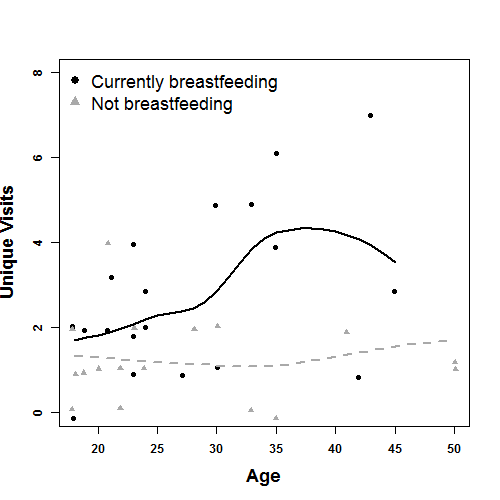
\includegraphics[width=0.75\textwidth]{bfeed_tot}
\caption{Please write your figure caption here}
\label{fig:1}       % Give a unique label
\end{figure}

\section{Discussion}
\label{sec:4}


%\begin{acknowledgements}
%If you'd like to thank anyone, place your comments here
%and remove the percent signs.
%\end{acknowledgements}

% BibTeX users please use one of
%\bibliographystyle{spbasic}      % basic style, author-year citations
%\bibliographystyle{spmpsci}      % mathematics and physical sciences
%\bibliographystyle{spphys}       % APS-like style for physics
%\bibliography{}   % name your BibTeX data base

% Non-BibTeX users please use
\begin{thebibliography}{}
%
% and use \bibitem to create references. Consult the Instructions
% for authors for reference list style.
%
\bibitem{RefJ}
% Format for Journal Reference
Author, Article title, Journal, Volume, page numbers (year)
% Format for books
\bibitem{RefB}
Author, Book title, page numbers. Publisher, place (year)
% etc
\end{thebibliography}

\end{document}
% end of file template.tex

